\section{Stan wiedzy w obszarze przedsięwzięcia}



\subsection{Rekonstrukcja}

Wirtualne reprezentacje krajobrazów miejskich są coraz bardziej wykorzystywane w różnego rodzaju zadaniach. Mimo rozwoju technik, począwszy od pozyskiwania danych (np. LiDAR), skończywszy na parametrycznych modelach (np. sieci neuronowe), zadanie modelowania pozostawia nierozwiązane problemy wpływające na jakość modelu wynikające z np. trudności akwizycji danych. 
Istnieje wiele sposobów rekonstrukcji które można podzielić ze względu na dane wejściowe, poziom szczegółowości, automatyzację czy też dane wyjściowe. W projekcie rekonstrukcja zachodzi na dwóch etapach - najpierw jako chmura punktów, następnie jako zbiór splatów. 

\subsubsection{Structure from motion}
Structure from motion (SfM)\cite{Schonberger_2016_CVPR} to technika fotogrametryczna służąca do szacowania struktur trójwymiarowych na podstawie zbiorów dwuwymiarowych obrazów, opierająca się na odnajdywaniu wspólnych punktów między obrazami. Jednym z wyróżnianych podejść jest inkrementalne SfM[\ref{fig:sfm_flow}], zawierające komponent iteracyjnej rekonstrukcji. Proces składa się z kilku kluczowych etapów:
\begin{enumerate}
  \item Ekstrakcja cech - przy wykorzystaniu algorytmów takich jak SIFT czy jego pochodne, zapewniających odporność na zmiany rotacji bądź oświetlenia, na każdym z obrazów wykrywane są punkty charakterystyczne, reprezentowane matematycznie przy pomocy deskryptorów;
  \item Dopasowywanie cech - pary obrazów testowane są pod kątem nakładania się sceny; punkty charakterystyczne z jednego obrazu są dopasowywane do odpowiadających im punktów na innych obrazach na podstawie podobieństwa deskryptorów;
  \item Weryfikacja geometryczna - SfM weryfikuje poprawność dopasowań cech, próbując oszacować transformację mapującą punkty między obrazami za pomocą geometrii rzutowej. Jeżeli transformacja odwzorowuje wystarczającą liczbę punktów, dopasowanie jest uznawane za zweryfikowane;
  \item Kroki rekonstrukcji inkrementalnej:
    \begin{itemize}
      \item \textbf{inicjalizacja} modelu oparta na wyborze pary obrazów o dużym pokryciu cech wspólnych,
      \item \textbf{rejestracja} kolejnych obrazów w modelu z wykorzystaniem dopasowań do punktów z już dodanych do niego obrazów, obejmująca szacowanie pozycji kamer,
      \item \textbf{triangulacja} nowych punktów występujących na przynajmniej dwóch obrazach zwiększająca pokrycie sceny i stabilność modelu,
      \item \textbf{regulacja wiązki} (\textit{ang. bundle adjustment}), czyli optymalizacja parametrów kamer i parametrów punktów minimalizująca błędy reprojekcji,
      \item \textbf{usuwanie punktów odstających}.
    \end{itemize}
\end{enumerate}
Głównymi wynikami procesu jest przeważnie zestaw wyznaczonych punktów 3D oraz obliczone pozycje i orientacje kamer.

\begin{figure}[!ht]
  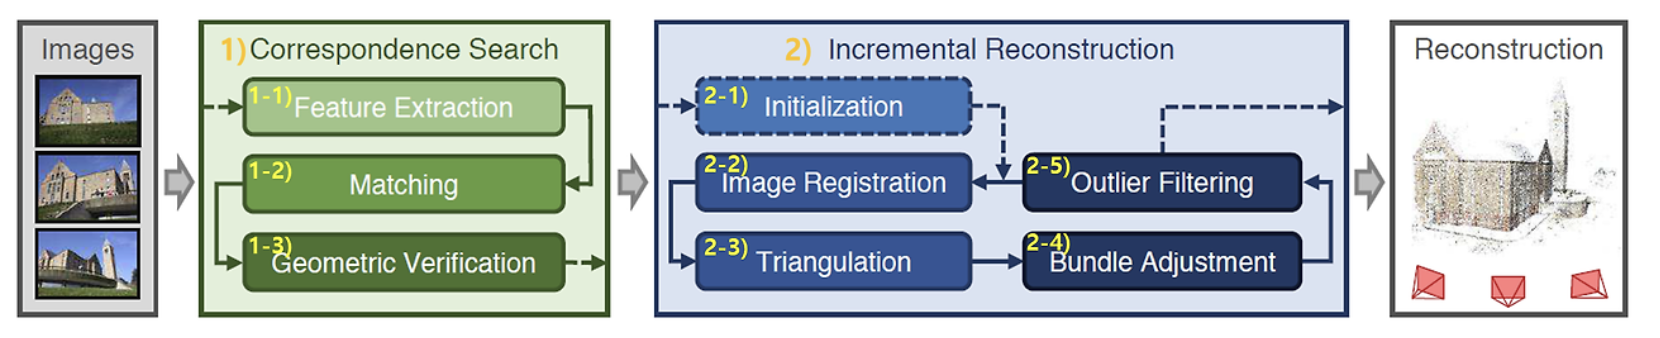
\includegraphics[width=\linewidth]{img/sfm_pipeline.png}
  \caption{Przepływ inkrementalnego SfM}
  \label{fig:sfm_flow}
\end{figure}

\subsubsection{Gaussian Splatting}

Popularną techniką rekonstrukcji z chmury punktów jest siatka (ang. mesh), wykorzystana np. w pracy City3D\cite{city3D}. Często jednak uzyskanie dobrej jakości siatki wymaga kombinacji wielu różnych geometrycznych algorytmów. Wraz z rozwojem sztucznej inteligencji zaczęły pojawiać się i w dziedzinie rekonstrukcji rozwiązania wykorzystujące sieci neuronowe - takie jak np. NeRF\cite{nerf}, gdzie informacje o scenie zawarte są w wagach modelu. Niedoskonałością tego rozwiązania jest jednak długi czas trenowania nawet dla sceny jednego obiektu, wahający się od parunastu godzin do paru dni. Z pomocą przychodzą inne metody, jak np. Gaussian Splatting \cite{gaussiansplatting}, który rezygnuje w całości z sieci neuronowej i wykorzystuje zbiór tzw. "splatów" do zbudowania sceny. Jako że w projekcie postawiono nacisk na optymalne wykorzystanie zasobów, to zdecydowano się na wybór właśnie ostatniej z wymienionych metod. 

\begin{figure}[!htb]
    % images need to be the same size
    \minipage{0.32\textwidth}
      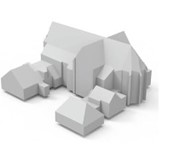
\includegraphics[width=\linewidth]{img/sota/city3dmesh.jpg}
      \caption{City3D - siatka}\label{fig:mesh_example}
    \endminipage\hfill
    \minipage{0.32\textwidth}
      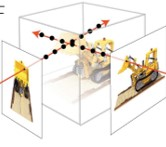
\includegraphics[width=\linewidth]{img/sota/nerfobject.jpg}
      \caption{Nerf - sieć neuronowa}\label{fig:nerf_example}
    \endminipage\hfill
    \minipage{0.32\textwidth}%
      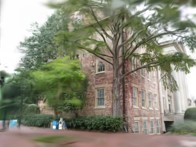
\includegraphics[width=\linewidth]{img/sota/gaussiansplattingobject.jpg}
      \caption{Gaussian Splatting - splat'y}\label{fig:gaussplat_example}
    \endminipage
\end{figure}

Splat (tłum. punkt rozmyty) jest rozszerzeniem punktu i posiada atrybuty
\begin{itemize}
    \item środek (x, y, z)
    \item kolor
    \item przeźroczystość
    \item macierz kowariancji (koduje rotację i skalę)
\end{itemize}

Najlepszy zbiór splatów opisujący scenę jest znajdowany w procesie optymalizacji opisanym poniżej schematem

\begin{figure}[!htb]
    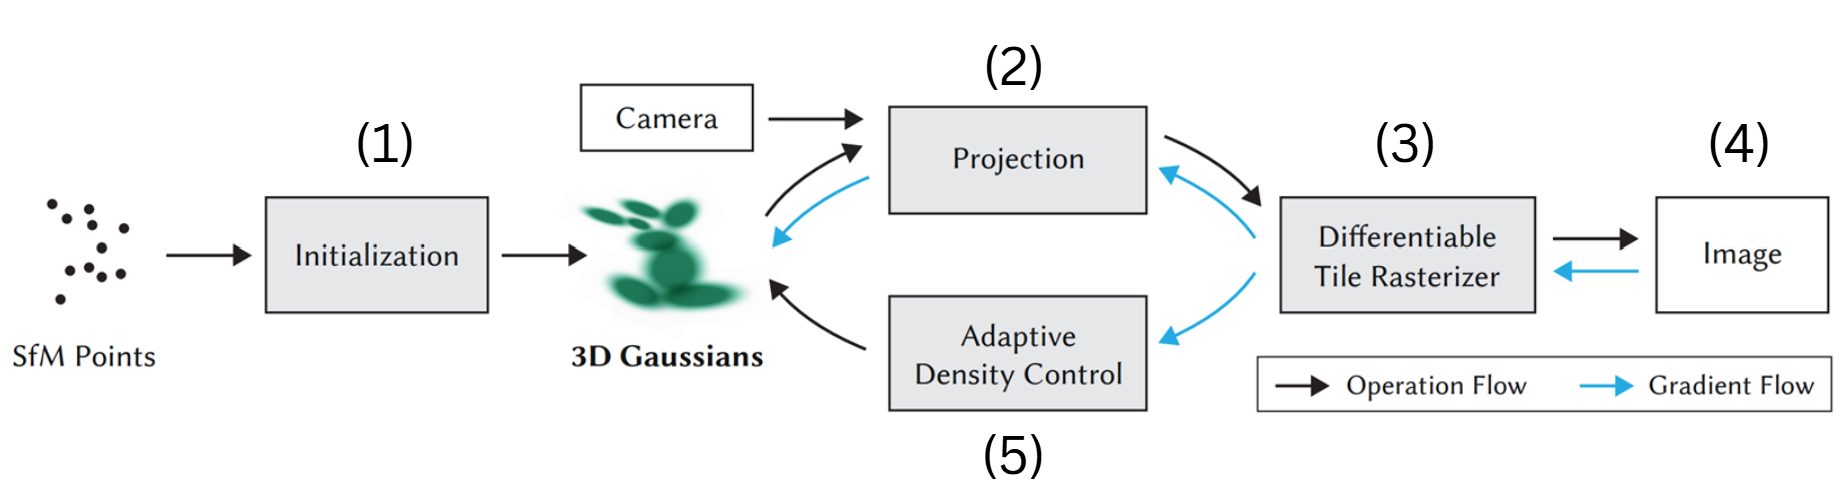
\includegraphics[width=\linewidth]{img/sota/gaussian_splatting_flow.png}
    \caption{Optymalizacja zbioru splatów}\label{fig:splatting_algorithm}
\end{figure}

\begin{enumerate}
    \item Wykorzystanie chmury punktów z rekonstrukcji do inicjalizacji zbioru splatów
    \item Rzutowanie perspektywiczne 3-wymiarowych gaussianów na obraz widziany z danej kamery, czego wynikiem jest zbiór dysków
    \item Renderowanie polegające na akumulowaniu dla każdego piksela wkładu od różnych nachodzących dysków 
    \item Obliczanie funkcji straty - porównanie z prawdziwym obrazkiem z danej kamery
    \item Adaptacja gęstości gaussianów - klonowanie, dzielenie lub usuwanie wg. kryteriów zależnych od strategii
\end{enumerate}

Niestety metoda ta nie pozostaje bez wad. W przypadku dużych zbiorów danych zużycie pamięci może wynieść nawet parę GB, co wymaga dobrej jakości karty graficznej. Inną kwestią jest duża liczba hiperparametrów, które często wymagają ręcznego dostosowania do danej sceny. 

\subsection{Segmentacja semantyczna}

Segmentacja semantyczna jest jednym z zadań uczenia maszynowego zaliczającym się do rodzajów segmentacji. Posiada ona cechy klasyfikacji, polega bowiem na przypisaniu każdemu z punktów w trójwymiarowej chmurze punktów odpowiedniej kategorii semantycznej, \textit{de facto} klasy. Punkty nie są więc traktowane osobno, a łącznie, co umożliwia na rozpoznanie zależności przestrzennych w chmurze punktów. W programie użyto na tym etapie projektu sieci neuronowych, jako rozwiązania szeroko używanego w rozwiązywaniu problemu segmentacji semantycznej obszarów miejskich.

\subsubsection{Architektura}

Istniejące z punktu widzenia architektury wyzwania wynikają ze specyfiki rozpatrywanych danych. Trójwymiarowe chmury punktów są zbiorami nieuporządkowanymi, nierzadko o różnej gęstości punktów w różnych obszarach chmury i różnej wielkości samej chmury. Cechy te wymuszają opracowanie specjalnych architektur adresujących ten problem.

Istniejące architektury sieci neuronowych dla zadania segmentacji semantycznej są przeznaczone głównie dla scen zamkniętych lub pojedynczych obiektów. Popularnym rozwiązaniem jest PointNet\cite{pointnet} oraz jego następca, PointNet++\cite{qi2017pointnetdeephierarchicalfeature} - obydwa oparte na wielowarstwowym perceptronie, jak i również bardziej skomplikowane rozwiązania jak KPConv\cite{thomas2019kpconvflexibledeformableconvolution} implementujące operację konwolucji użyteczną dla trójwymiarowych chmur punktów.

\subsubsection{Zbiór danych}

Ważnym problemem w uczeniu maszynowym jest dobór danych do efektywnego treningu modelu. W opracowywaniu naszego rozwiązania posłużyliśmy się otwartym zbiorem \textit{SensatUrban}\cite{hu2022sensaturban}. Zbiór ten zawiera wiele różnych chmur punktów z obszarami miejskimi w Anglii, o różnej wielkości. Każdemu z punktów przypisana jest jedna z 13 kategorii semantycznych reprezentujacych: podłoże, roślinność, budynek, ścianę, most, parking, tory, drogę, ławkę, samochód, chodnik, rower i obszary wodne. 